\documentclass[12pt,a4paper,norsk]{article}
\usepackage[norsk]{babel}
\usepackage[utf8]{inputenc}
\usepackage{natbib}
\usepackage{graphicx}
\usepackage{hyperref}

\usepackage[toc,page]{appendix} %For appendix og toc blargh.


\usepackage{pdfpages} %For å legge til vedlegg som pdf-filer

\usepackage{dirtytalk}
\usepackage{changepage}

\usepackage{nicefrac}

\usepackage{attachfile}
\usepackage{cleveref} %must be loaded last of the packages that modify LATEX’s referencing system.

\hypersetup{
    colorlinks,
    citecolor=black,
    filecolor=black,
    linkcolor=black,
    urlcolor=black
}

\title{IT1901 \\ Prosjektrapport}
\author{Gruppe 08\\
    755200, 741068, 757688,\\
    757676, 755591, 757787,\\
    757701, 757734, 757770}

\renewcommand{\contentsname}{Innhold}
\renewcommand\refname{Referanser}

\begin{document}
  \pagenumbering{gobble}
  \maketitle
  \newpage
  \pagenumbering{arabic}
  \tableofcontents
  \newpage
  \section{Introduksjon}

Dette prosjektet er et gruppeprosjekt gitt i emnet IT1901 - Informatikk prosjektarbeid 1, ved NTNU, høsten 2015. Målet med prosjektet og emnet er å gi deltagerne et innblikk i hvordan det er å jobbe med større gruppeprosjekter og  arbeidsmetoder hvor en tredjepart er med i prosessen. I dette prosjektets tilfelle er tredjeparten en kunde, som skal ta i bruk programmet. Prosjektet skal lære hvordan gruppeprosjekter gjennomføres og gi erfaringer rundt programmeringsverktøy, arbeidsmodeller og den smidige arbeidsmetoden \textit{Scrum}.

\subsection{Problemstilling}

Gruppen skal utvikle et administrasjonssystem for NTNUI Koiene. Systemet skal være et tillegg til NTNUI sine eksisterende websider, og gjøre det enklere å drifte koiene. Det skal for eksempel være mulig for en bruker å rapportere vedstatus og ødelagte ting, samt få beskjed om å ta med seg ting til en reservert koie. Medlemmer av Koiestyret skal kunne se disse rapportene og bruke de til å planlegge veddugnader og reparasjoner.

Dette programmet skal gruppen utvikle etter kundens ønsker og behov. Kunden har tildelt en rekke brukerhistorier som skal være oppfylt i det ferdige produktet.

\section{Gruppen og rutiner}
\subsection{Rutiner og timeplan}

Det første gruppen måtte løse var timeplanen for prosjektet. Ettersom en studentarbeidsuke er på 40 timer, og vi har 4 emner i semesteret, bestemte vi som gruppe for å møtes og jobbe sammen noe under 10 timer, fordelt på 3 dager i uka.

\begin{itemize}
  \item[] Mandager 9:15 - 11:00
  \item[] Torsdager 8:15 - 12:00
  \item[] Fredager 10:15 - 14:00
\end{itemize}

\subsection{Gruppen og ansvarsfordeling}
Gruppen bestemte seg tidlig for at alle skulle jobbe med forskjellige arbeidsoppgaver, men ikke låses i fastsatte roller. Dette gjorde vi for å dele kompetansen så mye som mulig og la alle få erfaring i de forskjellige aspektene ved prosjektet. På den måten får man gjort seg mindre avhengig av enkeltpersoner og får aktivisert gruppemedlemmer så mye som mulig.

  \section{Arbeidsprosess}
  \subsection{Scrum i teori}
  \textit{Scrum} er et rammeverk for å utvikle eller videreutvikle produkter, og er veldig populært innen software-utvikling. \textit{Scrum} er en smidig metode, og har som alle smidige metoder fokus på å respondere på endringer og samarbeid med kunden i løpet av prosjektets gang. [\cite{agilemanifesto}]

  I et utviklingsprosjekt har man gjerne to parter: kunde og utvikler-team. I \textit{Scrum} har man et \textit{Scrum}-Team med en produkteier, en \textit{Scrum}-master og utviklere (se avsnitt \cref{subsec:scrumroller} om \textit{Scrum}-roller). Produkteier er kundens representant i \textit{Scrum}-teamet. Produkteier jobber i samarbeid med utvikler-gruppen, ikke bare i planleggingsfasen av prosjektet, men også regelmessig under utvikling.
  [\cite{scrumguides}]
  \subsubsection{Produkt-backloggen}
  Produkteier stiller krav til prosjektet i form av en liste med brukerhistorier. Brukerhistorier er en kort forklaring av hva som skal kunne gjøres med et mål.  Brukerhistorier skrives ofte på formen “Som X skal jeg kunne Y for å Z”, hvor X beskriver brukertypen, Y handlingen brukeren skal kunne utføre og Z målet brukeren har med å utføre handlingen \cite[side 9]{kniberg}. Denne listen med brukerhistorier kalles for produkt-backloggen.
  %Hva menes med Mål?

    Backloggens brukerhistorier får en ID og et kort beskrivende navn. De blir vurdert fra viktigst til minst viktig, på bakgrunn av produkteiers prioriteringer og ønsker, men med eventuelle innspill fra utvikler-teamet.
  \subsubsection{Sprintplanleggingsmøtet}
  Utviklingsfasen deles opp i sykler, og blir i \textit{Scrum} kalt sprinter. I begynnelsen av hver sykel har man i \textit{Scrum} et sprintplanleggingsmøte. Deltakerne på møtet er ikke bare medlemmer av utviklingsteamet med \textit{Scrum}-master, men også produkteier. Formålet med møtet er å forberede og justere produkt-backloggen og planlegge neste sprint.

    \textit{Scrum}-teamet avgjør hvor lang sprinten skal være og finner ut hvilke ressurser man har på denne sprinten. Gruppen avtaler tidspunkt for når på dagen gruppen skal ha det daglige \textit{Scrum}-møtet, når retrospektiv-møtet for sprinten skal være og når demonstrasjonen for produktet skal være \cite[side 16]{kniberg}.

  \subsubsection{Release-plan}
  I noen prosjekter kan det være hensiktsmessig å planlegge lengre frem i tid enn kun for den neste sprinten. Man lager en releaseplan for hele prosjektet. Hensikten med denne er å gjøre det samme som i sprintplanleggingsmøtet, men for alle brukerhistorier. Etter at en sprint er ferdig har man et sprintplanleggingsmøte der man justerer release-planen utifra eventuelle endringer og hvordan sprinten faktisk gikk \cite[side 95 - 101]{kniberg}.

  \subsubsection{Daglig Scrum}
  I \textit{Scrum} har man et daglig møte der hver person svarer på de tre spørsmålene:

  \begin{itemize}
        \item[1.] Hva gjorde jeg sist gang som hjalp gruppen å nå sprintmålet?
        \item[2.] Hva skal jeg gjøre i dag for å hjelpe gruppen å nå sprintmålet?
        \item[3.] Ser jeg noen eventuelle utfordringer for meg eller gruppen, som kan hindre oss i å nå sprintmålet?
    \end{itemize}

    \textit{Scrum}-møtet skal være kort, med fokus på å få hjelp om man har noen utfordringer.

  \subsubsection{Retrospektiv-møtet}
      Retrospektive møter en en viktig del av \textit{Scrum}. Retrospektiv-møtet er gruppens mulighet til å forbedre prosesser og arbeidsrutiner. Retrospektiver har man på slutten av hver sprint, og både utviklingsgruppen, \textit{Scrum}-master og produkteier deltar. På møtet diskuterer man og svarer på følgende spørsmål:

  \begin{itemize}
        \item[1.] Hva gikk bra i løpet av denne sprinten?
        \item[2.] Hva gikk mindre bra i løpet av denne sprinten?
        \item[3.] Hva kan gruppen gjøre bedre neste sprint?
    \end{itemize}

    Det siste punktet er det som er hovedfokuset i møtet. Det er viktig å komme med konkrete eksempler slik at man er helt sikker på hva det er man kan endre på til neste gang. Retrospektiv skal være den tryggeste måten for gruppen å få frem sin mening, det er derfor viktig at alle i gruppen blir hørt og at ingen skal føle at de ikke kan si sin mening. En måte å få til dette på er at man én etter én får si sin mening om sprinten, uten at andre avbryter eller kommer med kommentarer til det som blir sagt. Etter at alle har fått sagt det de vil, så kan man diskutere i gruppen hva som er viktigst å fokusere på og forbedre neste sprint.

    Disse møtene er viktig fordi det alltid er rom for forbedring i alle grupper. Hvis man ikke har et oppsatt møte der man tar opp hva som har skjedd i sprinten så vil man gjøre akkurat de samme feilene i den neste. Dette gir gruppen muligheten til å forbedre seg utover prosjektet.
    \cite[side 82 - 88]{kniberg}
  \subsubsection{Scrum-roller}\label{subsec:scrumroller}
  \textbf {Produkteier}
    \par Produkteier er kundens og eventuelle andre interessenter sin representant. Vedkommende er ansvarlig for å oppdatere  produktbackloggen og for å kommunisere til utviklerne hva brukerhistoriene innebærer.
    [\cite{scrumguides}]

    \bigskip \noindent \textbf{\textit{Scrum}-master}
    \par En \textit{Scrum}-master er en tilrettelegger for et produktutviklingsteam som bruker \textit{Scrum} som utviklingsmetodikk, som gir teamet muligheter for selvorganisasjon og håndtering av plutselige endringer under prosjektet. I tillegg til det bruker han/hun \textit{Scrum} for å effektivisere hele arbeidsprosessen og er ansvarlig for at \textit{Scrum} blir brukt som tiltenkt.

    \begin{itemize}
    \item[-] Hjelper med å rekke sprintmålene.
    \item[-] Støtter produkteieren med å oppdatere backloggen ved potensielle endringer underveis slik at teamet kan reagere på de.
    \item[-]  Hjelper teamet med å finne en eksplisit definisjon for “done” med vurdering av innspill fra kunden.
    \item[-]  Lærer bort \textit{Scrum}-teknikker til teamet for å sikre at produktet leveres med høy kvalitet.
    \item[-]  Hjelper teamet med å jobbe mer selvstendig.
    \item[-]  Hjelper teamet med å identifisere og unngå eller fjerne             potensielle og faktiske kilder for forstyrring og hindring for både interne og eksterne kilder.
    \end{itemize}

    [\cite{scrummaster}]
    [\cite{scrummasterrolle}]

    \bigskip \noindent \textbf{Utviklere}
        Medlemmene av utvikler-gruppen har ansvar for å gjøre produkt-backloggen om til et fungerende produkt. Utviklere er ikke delt inn i delgrupper. Medlemmer kan ha forskjellige fokusområder, men alle har like mye ansvar for produktets kvalitet. Utviklere ledes ikke av \textit{Scrum}-master, men får hjelp til å være selvorganiserende.

  \subsubsection{Task-board}
  Task-boardet er et verktøy for å gjøre hele arbeidsprosessen mer oversiktlig og interaktiv. Man kan se hvilke brukerhistorier og deloppgaver som må gjøres for sprinten, om de er delegert, om de er ferdige og hvilken prioritet de har. Figur \ref{fig:task-board} viser et eksempel-task-board.

    \begin{figure}[h!]
    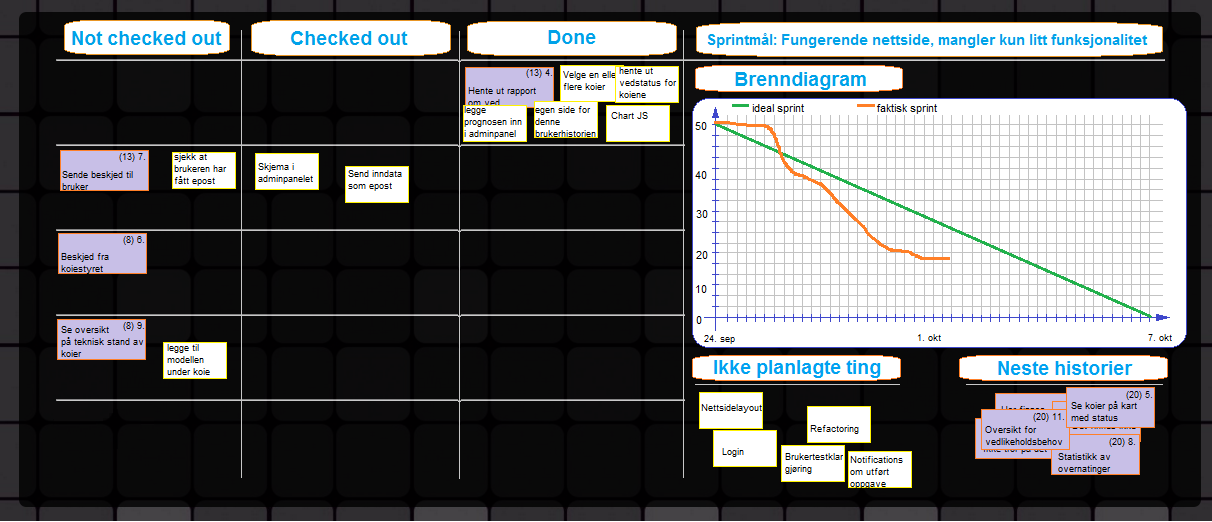
\includegraphics[width=\linewidth]{img/task-board.png}
      \caption{Eksempel på task-board med brenndiagram}
      \label{fig:task-board}
  \end{figure}

    \textit{Task-boardet} er delt inn i 4 kolonner: \textit{Not checked out}, \textit{Checked Out}, \textit{Done} og \textit{Sprintmål}.

    \textit{Not checked out}: Her er brukerhistoriene ingen har startet på enda. Brukerhistoriene er sortert etter viktighet. De viktigste står på toppen. Historiene er splittet i flere mindre oppgaver.

    \textit{Checked out}: Her er brukerhistoriene, deloppgavene og “ikke planlagte ting” (se avsnitt om Ikke planlagte ting) som allerede jobbes med.

    \textit{Done}: Når en brukerhistorie er ferdig, ender den og alle deloppgaver her. Alle som jobber med prosjektet vet da at denne historien oppfyller kravene som er nødvendig for at den kan kalles for “ferdig/done”.

    \textit{Sprintmål}: Her vises sprintmålet og en seksjon som er delt i tre: Brenndiagram, Ikke planlagte ting og de neste historiene i produkt-backloggen.

    \paragraph{Brenndiagram:}
    Et todimensjonalt diagram der x-aksen viser datoene mellom sprintstarten og sprintslutten. Y-aksen viser arbeidet som er igjen i storypoints. En tegner en graf ut fra hvor man er i sprinten (dato) og hvor mange deloppgaver/brukerhistorier som er blitt fullført denne dagen. Dersom tidsestimatene er riktige ender man opp med en graf som går fra diagrammets venstre topp til høyre bunn i en nesten rett linje.

    \paragraph{Ikke planlagte ting:}
    Her finnes deloppgaver som dukker opp underveis. Disse var ikke planlagt fra starten, men må implementeres for at produktet skal fungere. Ved for dårlig planlegging, kan dette føre til en flom av ikke planlagte elementer. Arbeidsmengden vil da øke raskere og det ender med en for sakte synkende graf.

    %Høres ut som.. "hvordan tolke brenndiagrammet"...
    %Trenger vi dette? TODO: make up our hive-mind.
    Faresignaler fra brenndiagrammet kan være: Hvis grafen synker for fort, har brukerhistoriene tatt mindre tid enn forventet, dette skyldes dårlig estimering. Synker grafen for sakte har estimatene vært for lave. Disse problemene løses motsatt, synker grafen for fort flyttes brukerhistorier fra "neste historier" og inn i sprint, synker den for sakte flyttes brukerhistorier inn i "neste historier".

    \paragraph{Neste historier:}
    Her er alle brukerhistoriene som ikke er implementert enda og ikke har fått plass i den nåværende sprinten.

    \cite [side 72 -78]{kniberg}


  \subsubsection{Utviklingsverktøy}

%\textbf{PyCharm}
%\par De fleste på gruppen brukte PyCharm for å jobbe med pythonfilene. PyCharm er en IDE som er mye brukt i programutvikling siden det har mange flere funksjoner enn en vanlig teksteditor som gjør jobben enklere. I tillegg er det mulig å teste koden med en gang i konsollen, samt at GIT kan brukes i selve programmet for å holde prosjektet oppdatert.

\bigskip \noindent \textbf{GIT og Stash}
\par For å holde orden på versjoner og endringer i prosjektet brukte vi GIT koblet opp til Stash for å forsikre oss om at ingen endringer og oppdateringer gikk tapt. På Stash hadde vi et repository, dette er et område der all koden til prosjektet blir lagret. Repositoriet var delt opp i branches, der forskjellige versjoner av koden lå lagret adskilt. Master var selve hovedbranchen hvor nåværende produkt lå. Hver gang noen skulle lage en ny ending i produktet, så ble det laget en ny sidebranch, denne ble så merget med masterbranchen når endringen var ferdig. Dette gjør at det er mulig at flere personer jobber med samme kode på forskjellige maskiner samtidig, uten at det blir gjort feil.

I tillegg til at man kan ha flere branches, vil man trenge godkjenning av andre gruppemedlemmer for å merge en ny branch inn i master. Slik kan man være sikrere på at feil i koden blir plukket opp tidlig. Alle endringer som har blitt gjort på prosjektet blir også lagret, så om noe virkelig går galt er det mulig å gå tilbake til en tidligere versjon og å gjøre ting på nytt.


  \subsection{Scrum i praksis}
    Det vil omtrent aldri være mulig å overføre teori direkte til praksis. Kniberg skriver i introen til \textit{Scrum and XP from the trenches} \cite[side 2]{kniberg}:

    \bigskip\begin{adjustwidth}{2.5em}{0pt}
    \say {\textit{The strength and pain of Scrum is that you are forced to adapt it to your specific situation}}
    \end{adjustwidth}
    \bigskip Gruppens største utfordring med å tilpasse Scrum var på grunn av forskjellige timeplaner og mangel på et fast og privat rom. I motsetning til en prosjektgruppe i et konsulentfirma ville vi ikke ha muligheten til å møtes hver dag i uka på samme sted.

  \subsubsection{Sprintlengde}
  Gruppen bestemte seg for at 2 uker lange sprinter var praktisk fordi vi da kunne møte med veileder for prosjektet midt i sprinten og produkteier i slutten. Korte sprinter ville gjøre det mulig for oss å ha retrospektive møter ofte og få tilbakemelding fra produkteier om vi er på rett spor. I slutten av hver sprint var planen å teste funksjonene som hadde blitt implementert i sprinten med produkteier. Dette i form av en brukbarhetstest med scenario-tester.

    Med to uker lange sprinter ville vi oppnå 4 sprinter i løpet av prosjektperioden, med avslutning 4. november. Ettersom innlevering av rapport hadde frist 12. november ville vi ha mulighet etter siste sprint til å jobbe med ferdigstilling av rapporten.

    De timene vi planla å jobbe med hver uke ble delt inn i økter for å estimere arbeidskapasitet per sprint. Denne enheten var også den vi ville bruke når vi skulle estimere hvor mange storypoints en brukerhistorie krevde - 1 økt = 1 storypoint. I løpet av en uke ville en person ha 5 økter: mandag: 1, torsdag 2, fredag: 2. Ettersom vi var en gruppe på 9 personer ville vi ha sprinter med 9 (personer) x 5 (økter pr uke) x 2 (uker) = 90 økter pr. sprint. Vi anslo at av 90 teoretiske økter i løpet av en sprint ville ca. 50 økter bli brukt på brukerhistorier. Tallet er lavere siden noen økter går til møter i gruppen eller med produkteier, mens andre går til rapportskriving, oppsett av utviklermiljø, tid til å sette seg inn i rammeverk eller forbereding til demonstrasjoner og tester. Vi antok at mye av tiden av vår første sprint kom til å gå til planlegging av prosjektet og sette opp utviklermiljø, og anslo at produktive økter kom til å være på ca. 25 økter. Sprint 2,3 og 4 anslo vi til 50 arbeidsøkter, fordi vi antok at vi da kom til å være satt opp med prosjektet, kommet inn i bruk av \textit{Scrum} og klare til å bruke mer tid på utvikling, og mindre tid på administrativt arbeid.

  \subsubsection{Brukerhistorier}
  Produkteier rangerte brukerhistoriene og ga dem lav, høy eller vanlig proritet. Deretter måtte vi rangere historiene igjen, for å finne hvilke vi skulle implementere først av de med høyest prioritet. Noen historier så ut til å være avhengige av at andre var ferdige, og måtte nødvendigvis havne i tilsvarende rekkefølge. På grunn av estimater på noen historier måtte vi også gjøre en brukerhistorie med lavere prioritet før en med høyere prioritet, fordi det var den eneste vi fikk plass til i sprinten.

    Når vi skulle estimere hvor mange arbeidsøkter en brukerhistorie kom til å ta, brukte vi planning poker på hver brukerhistorie. Planning poker utføres ved at hver gruppemedlem får en kortstokk med 13 kort, med verdiene 0, \nicefrac{1}{2}, 1, 2, 3, 5, 8, 13, 20, 40, 100, ?, “Pause”. Alle velger individuelt ett av kortene som representerer estimert tid for å løse brukerhistorien. Har man bestemt seg for et kort skal det legges på bordet slik at estimatet er skjult. Når alle har et kort liggende foran seg er det på tide å snu dem. Dersom det oppsto store avvik i estimert tid skal man diskutere hvorfor estimatene blir så forskjellige. Deretter skal brukerhistorien estimeres igjen for å se om gruppen blir mer enige om estimatene \cite[side 38-40]{kniberg}.

    Det viste seg å være nyttig. Vi fikk da avdekket at det var forskjellige oppfatninger i gruppen av hva slags tekniske implikasjoner historien innebar. Når en historie ga vidt forskjellige verdier, så kunne de som mente at historien trengte få økter få si hvorfor de mente den ikke trengte så mange og motsatt med de som mente historien trengte mange. Allerede da kom det opp mange gode forslag på hvordan brukerhistorier kan løses på et teknisk nivå. Noen i gruppen visste allerede litt om hva slags muligheter vårt valgte rammeverk ga, og hadde allerede ideer på hvordan spesifikke ting kunne løses. Når vi tok en ny runde planning poker på den samme brukerhistorien fikk vi likere resultat og kunne fastsette antall økter på en brukerhistorie.

  \subsubsection{Vårt Task-board}
  Gruppen bestemte seg for å organisere task-boardet via "Trello.com". Trello er et web-verktøy som kan brukes som et digitalt task-board. Alle på gruppen lagde seg en trellobruker, og vi lagde et team som alle på gruppen ble medlem av. Vi inviterte også produkteier til å bli medlem av teamet, så produkteier kunne ha oversikt over hvordan vi lå an, og skrive inn prioriteringer på brukerhistoriene.

    I Trello kan man lage forskjellige brett, noe vi gjorde for hver sprint. På hvert respektive brett la vi til lister med kort, der hvert kort representerte en brukerhistorie. For hvert brett ble det laget lister for “Not checked out”, “Checked out”, “Andre oppgaver som dukker opp underveis” og “Done”. Etter releaseplanleggingen ble brukerhistoriene lagt inn som kort i “Not checked out” for alle sprintene.

    Når noen skulle begynne på en brukerhistorie, ble det tilsvarende kortet flyttet over til checked out. Trellobrukerne til de som jobbet med brukerhistorien ble knyttet opp mot kortet, så det ble lett å se hvem som jobbet med hva.

    Utvidelsen \textit{Burndown for Trello} lot oss legge inn estimert tidsbruk og storypoints på et kort, hvor mye tid som faktisk ble brukt på hvert kort, og automatisk generere brenndiagram basert på de to. Se vedlegg ~\ref{app:taskboard} for forklaring på hvordan vi brukte Trello som task-board.
  \subsubsection{Våre Retrospektiver}

\bigskip \noindent \textbf{Retrospektiv Sprint 1}
\par Dagen etter første sprint hadde gruppen sitt første retrospektivt. Gruppen  diskuterte hvordan første sprint hadde gått. Gruppemedlemmene fikk hver sin tur til å si: “Hva som gikk bra”, “Hva som gikk dårlig” og “Hva vi kan forbedre” (se vedlagt møtereferat: ~\cref{app:sprint1}).

\paragraph{Hva gikk bra:}
I den første sprinten var gruppen mer effektiv enn vi hadde regnet med, dette resulterte i at gruppen fikk fullført flere brukerhistorier enn antatt. Samarbeidet i gruppen fungerte veldig bra, spesielt var gruppemedlemmene flinke til å hjelp hverandre.Fordelingen av arbeidsoppgaver gikk lett, gruppen delte seg opp i mindre grupper som tok ansvar for hver sine arbeidsoppgaver. Gruppemedlemmene var også flink til å dele kunnskapen med hverandre. En måte gruppen delte kunnskap var ved bruk av \textit{parprogrammering} \cite[side 17]{dyba}, der små grupper kodet sammen. Et av gruppemedlemmene skrev koden mens resten hjalp den som kodet. Denne metoden lot de som ikke var helt komfortable med teknologiene som ble brukt, bli bedre kjent med teknologiene mens de kunne støtte seg på andre grupemedlemmer. Gruppens medlemmer var også flinke til å tilegne seg ny kunnskap på egenhånd.


\paragraph{Hva gikk ikke bra:}
På første møte bestemte gruppen at det ukentlig skulle være sosiale samlinger, dette var for å bli bedre kjent og for å få en pause i lange arbeidsøktene. Den sosiale samlingen ble bestet til å være pizza på fredager. Dette ble ikke gjennomført den første sprinten
Gruppen hadde litt sykdom og annet frafall i løpet av sprinten.
Gruppen satte av tid for å sette opp utviklingsmiljøene og til å lære seg verktøyene som skulle brukes i prosjektet. Til tross for dette oppstod det problemer med flere av utviklingsmiljøene i løpet av sprinten. Problemene med utviklingsmiljøene var en uberegnet faktor som tok ekstra tid.

På grunn av problemene med utviklingsmiljøene og mangel på oppgaver, var det til tider vanskelig å syslsette alle gruppemedlemmene.

Fordeling av arbeidsoppgaver på grupper førte til at ikke alle gruppemedlemmen fikk satt seg inn i de samme teknikkene.
Gruppen underestimerte arbeidet gruppen fikk gjort.


\paragraph{Hva kan forbedres:}
Inkludere alle i gruppen i flere av oppgavene, samt passe på at medlemmene i gruppen har noe å jobbe med.
Inkludering i flere oppgaver fører til at alle får kodet og jobbet med rapporten.
Grupppen må også passe på å ta gjevnlige pauser.
Gruppen må ta tid til sosialisering.
Loggføring av arbeid og timer på arbeidsoppgaver må skjerpes for å gjøre det lettere å lage brenndiagram.
Gruppen kom også frem til at gruppen skulle lage en risikoplan for prosjektet, slik at gruppen var forberedt på forutsigbare hendelser.



\bigskip \noindent \textbf{Retrospektiv Sprint 2}
\par Gruppen hadde retrospektiv dagen etter demo for sprint to, hvor gruppen gikk igjennom de samme tre spørsmålene som i første retrospektiv, (se vedlagt møtereferat: ~\cref{app:sprint2}).

\paragraph{Hva gikk bra:}
En av tingene gruppen skulle forbedre fra forrige sprint var å gi alle i gruppen er oversikt over prosjektet. Gruppen var flinkere til å inkludere flere medlemmer i flere oppgaver, som førte til bedre forståelse av kode og bedre oversikt over prosjektet i helhet for alle gruppemedlemmer. En annen konsekvens at alle ble inkludert i flere oppgaver var at arbeidsoppgavene ble bedre justert til gruppemedlemmene.

I løpet av sprinten hadde gruppen fokus på teambuilding. Vi tok en pause fra arbeid og spiste pizza sammen hver fredag, en “tradisjon” som vi fortsatte med. Innimellom på møtene prøvde vi også å gjøre noe morsomt sammen, som å se videoer på youtube i pausene.
Generelt er inntrykket at vi jobber bra som en gruppe og ligger godt an.
I denne sprinten fikk vi gjort mer enn  koding i prosjektet, vi fokuserte mer på administrative oppgaver og rapporten. Vi laget risikoanalyse, utbedret testplanen og har skrevet på rapporten.

\paragraph{Hva gikk ikke bra:}
I slutten av sprinten fant vi ut at vi hadde litt for stor arbeidsmengde. Det gjorde at vi måtte overføre noen deloppgaver på ene brukerhistorien til den neste sprinten.
Et problem som vi merket denne sprinten var at vi fikk mindre ressurser å jobbe med. Det var større fravær, ved sykdom og høstferie. Dermed ble arbeidsmengden større enn normalt, i tillegg til at gruppemedlemmer oftere dukket opp seint, slik at det tok lengre tid å komme igang med møtene.

\paragraph{Hva kan forbedres:}
Siden mange var borte denne sprinten så ble gruppen enig om å bli bedre på å finne seg arbeidsoppgaver å gjøre hjemme ved frafall.
I tillegg så skal vi ha en person som følger opp de som er borte/seine og ha 1-1 samtaler med dem for å finne bedre ut hvorfor de er seine og hvordan det kan unngås.


\bigskip \noindent \textbf{Retrospektiv Sprint 3}
\par Etter den tredje sprinten hadde vi et retrospektivt møte før vi begynte neste sprint, (se vedlagt møtereferat: ~\cref{app:sprint3}). Da gjorde vi det samme som i de forrige retrospektivmøtene.

\paragraph{Hva gikk bra:}
Flere i gruppen har tatt mer ansvar for sitt eget arbeid, har vært flinkere til å finne seg oppgaver å gjøre og å være mer engasjert i prosjektet. Spesielt har det gått bra å jobbe hjemmefra når noen i gruppen har vært syk, kommunikasjonen mellom de som har vært borte og gruppen har vært så bra at dette har gått smertefritt. Dette viser god forbedring fra forrige sprint da vi ville bli bedre på akkurat dette, mye fordi vi har hatt en person som følger opp de som er borte.
Gjennom sprinten så har gruppen vært effektiv med arbeidsoppgavene, det vises ved at de oppgavene som var igjen fra forrige sprint, de fra denne sprinten og deler av neste sprint ble fullført. Dette er fordi alle har vært flink til å finne enkle løsninger på oppgavene.
%I tillegg til brukerhistorier og design har gruppen også gjort noe morsomt på nettsiden med noen gjemte funksjoner, også kalt “easter eggs”.

\paragraph{Hva gikk ikke bra:}
En av tingene som gikk dårlig i denne sprinten var estimater av tid på brukerhistoriene, vi regnet med å bruke lengre tid på dem. Dette var fordi ingen hadde god nok kjennskap til de ulike verktøyene som skulle brukes til å gjøre et mer riktig estimat, f.eks. for å lage kart på en nettside.
I sprinten var det dårlig fokus på å føre timer som ble brukt på de forskjellige oppgavene og å skrive logg for hva som skjedde på hvert møte.
Flere i gruppen ble syk og var borte flere ganger enn tidligere, men en i gruppen tar alltid kontakt hvis noen er borte og ikke gir beskjed, slik kan de få oppgaver å gjøre hjemme.
Mot slutten av sprinten så var mye av arbeidet ferdig, da var det generelle inntrykket i gruppen at alt var ferdig. Det gjorde at man slappet litt mer av og ikke jobbet like hardt som var ønskelig, iallefall siden det viste seg at det var problemer med noen av funksjonene som vi måtte fikse i neste sprint.
Når det kom til rapporten så mente flere i gruppen at det var vanskelig å vite hvordan man skulle skrive en bra rapport, det førte til at deler av rapportskrivingen gikk sakte da man satt seg fast.

\paragraph{Hva kan forbedres:}
Vi har sett tidligere at en logg for hvert møte kan være bra for dem som er borte en dag så de får oversikt over hva som har blitt gjort mens de var borte. Selv om denne kommunikasjon har gått bra denne sprinten så er det fortsatt ønskelig å ha en logg til senere, så dette er et punkt gruppen må bli bedre på til neste sprint.
Et annet punkt gruppen kan bli bedre på er å holde de møtene vi har fokusert på de oppgavene som må gjøres, til tider hender det at fokuset drifter over på ting som ikke er så viktig. Siden det fortsatt er mye fravær og forseintkomminger så ville det vært bra for gruppen at alle blir flinkere til å komme til tide, kanskje ved å sette på 2 alamer på morgenen.
Noe som er veldig viktig er at man tester funksjoner bedre før man skriver at de er ferdig, da slipper gruppen å tro at alt er ferdig når det fortsatt er feil i funksjoner.


\bigskip \noindent \textbf{Retrospektiv Sprint 4}
\par Etter den tredje sprinten hadde vi også et retrospektivt møte før vi begynte neste sprint, (se vedlagt møtereferat: ~\cref{app:sprint4}). Da gjorde vi det samme som i de forrige retrospektivmøtene.

\paragraph{Hva gikk bra:}
I denne sprinten ble vi helt ferdig med produktet, selv om det ikke var mange oppgaver igjen til denne sprinten så er gruppen godt fornøyd med å være ferdig. Dette har vi gjort ved å ha god arbeidsånd mot slutten av prosjektet, det har vært godt oppmøte og mye har blitt gjort.
Gruppen er også fornøyd med hvor mye som er ferdig på rapporten, og det merkes at det har blitt gjort arbeid på den i tidligere sprinter også.

\paragraph{Hva gikk ikke bra:}
Noe gruppen ikke var forberedt på var at det skulle skrives dokumentasjon på all koden, dette var ikke en del av planen vi la opp mot slutten av prosjektet.
Selv om vi har jobbet godt og fått gjort mye så har det til tider vært litt dårlig fokus og tull på møtene. En grunn til dette er at mot slutten av prosjektet begynner folk å bli litt lei og slitne, spesielt når man sitter og skriver rapport i lengre perioder. Gruppen merket til tider at 4 timer i strekk var litt for lange arbeidsmøter, derfor ble de kuttet ned til 2 timer.
Et problem med å skrive rapport er at vi har skrevet over maksgrensen for ord, som kan føre til at det er noe irrelevant og duplisert arbeid.

\paragraph{Hva kan forbedres:}
En ting gruppen kunne forbedret var å involvere flere personer i rapportskriving tidligere, slik at det ikke ble like mye å gjøre mot slutten.
Gruppen skulle også klart å holde bedre fokus på møtene, for å være enda mer effektive.
En annen ting vi kunne gjort bedre var å endre arbeidsmetoden i denne sprinten, der det for det meste bare var rapportskriving. Fordi måten man jobber best med kode og rapport er ikke nødvendigvis det samme, f.eks. lengde på arbeidsøkter, og man kan gjøre mer hjemme og møtes færre ganger.

  \subsubsection{Sprintgjennomgang}
\bigskip \noindent \textbf{Sprint 1}
\par Sprint 1 startet med et sprintplanleggingsmøte der det ble diskutert hva som  skulle gjøres i sprinten og hvilke brukerhistorier vi skulle utføre. Disse ble valgt etter hva kunden hadde satt opp som høy prioritet. (Ref: \cref{app:releaseP3}) Gruppen laget også en brukerhistorie, administrasjon av koiene på nettsiden, som ble satt til sprint 4 siden det ble antatt at den kom til å ta lang tid.

Halvparten av arbeidsøktene i sprinten var satt til å sette opp Stash installere PyCharm og å laste ned Django. Administrasjonsdelen og starten av nettsiden ble også laget. Dette tok ikke like lang tid som var estimert og gjorde at det ble mer tid til å kode brukerhistoriene.

Da brukerhistoriene ble startet, delte gruppen seg opp i to og gjorde en brukerhistorie hver. Begge brukerhistoriene handlet om å rapportere ting, \textit{ved} og \textit{ødelagte ting}. De var veldig like så alle på gruppa kunne lære seg det grunnleggende og hjelpe hverandre med det som var vanskelig.  Disse brukerhistoriene tok noe lenger tid enn estimert siden alle var nybegynnere. Dette jevnet seg ut etterhvert i sprinten.

Den siste brukerhistorien i sprinten, \textit{koiestyret skal kunne ta ut rapporter av ødelagte ting}, tok mye mindre tid enn estimert, fordi det bare var å koble rapporterte ting til admin-panelet. Gruppen fikk derfor tid til overs og valgte å overføre brukerhistorien om å rapportere inn tekniske utbedringer på en koie fra sprint 2 til 1. Denne hadde lavere prioritet, men lavt nok tidsestimat til at man ville rekke å fullføre den.

Brenndiagrammet viser hvordan progresjonen for oppgavene var i denne sprinten (se vedlegg, sprint1: \cref{app:brenn}).

\bigskip \noindent \textbf{Sprint 2}
\par Sprinten startet med et sprintplanleggingsmøte. Vi gikk ut fra releaseplanen, men siden en av brukerhistoriene ble flyttet til sprint 1 ble det hentet en fra sprint 3 (se vedlagt releaseplan-v2: ~\cref{app:releaseP3}). Gruppen valgte brukerhistorien med likest tidsestimat til den som ble flyttet til sprint 1. Gruppens egenlagde brukerhistorie om \textit{administrasjon av koiene} ble implementert av seg selv da andre oppgaver ble gjort, så den ble ikke arbeidet spesifikt på og ble derfor fjernet. Gruppen valgte å lage enda en brukerhistorie, der nettsiden skulle designes med forside og navigering. Dette gjenspeiler målet for sprinten; "Ha en fungerende nettside som kun mangler litt funksjonalitet".

I denne sprinten handlet brukerhistoriene om direkte kontakt mellom koiestyret og brukere, og det å ta ut rapporter for ved og teknisk stand. Her ble oppgavene fordelt på mindre grupper. Funksjonene for vedrapporter og teknisk stand gikk bra, fordi det lignet det som ble gjort i forrige sprint.

Den viktigste brukerhistorien i sprinten var å kunne ta ut ved vedrapporter og -prognoser for koiene. Den var litt vanskeligere, dette var fordi man selv måtte definere hvor mye ved som gikk når koien ble brukt og så lage en graf ut av dette og en prognose for når det blir tomt.

I denne sprinten ville gruppen fullføre brukerhistoriene som handlet om kommunikasjon mellom koiestyret og brukeren, derfor ble et epostsystem for å melde fra om ting som måtte tas med til og fra koier implementert.

Arbeidet med nettsiden kom ganske langt, det ble laget forside og en navigasjonsmeny der de funksjonenene som var laget ble lagt til. Nettsiden fikk derfor mye funksjonalitet veldig tidlig, blant annet å kunne melde inn ved, ødelagte ting og tekniske utbedringer fra brukeren, og at koiestyret kunne hente ut rapportene.

I slutten av sprinten ble det funnet noen bugs i vedprognosefunksjonen som det ikke ble tid til å fikse, disse ble derfor overført til neste sprint.

Brenndiagrammet viser hvordan progresjonen for oppgavene var i denne sprinten (se vedlegg, sprint2: \cref{app:brenn}).

\bigskip \noindent \textbf{Sprint 3}
\par Sprinten startet med et sprintplanleggingsmøte. Vi gikk ut fra releaseplanen (se vedlegg releaseplan-v3: ~\cref{app:releaseP3}). I denne sprinten var det kun 2 brukerhistorier, men tidsestimatet på dem var veldig høyt. I tillegg til disse hadde gruppen oppgaver fra forrige sprint, og en del arbeid med å få nettsiden til å se ferdig ut. Det ble også holdt en demonstrasjon av produktet.

Brukerhistorien om oversikt over vedlikedholdbehov utfra forventet levealdre på konstruksjonen av koien var det noe usikkerhet rundt. Måtte man gå gjennom alle koiene og finne ut når de ble bygget og oppusset, og når de må gjøres noe med? Etter å ha snakket med kunden kom man frem til en bedre løsning der man istedenfor legger inn når noe er reparert/satt inn nytt og hvor lenge disse vil vare, så kan man se på nettsiden når de må gjøres noe med igjen.

Brukerhistorien om kart over koiene med ved- og utstyrsstatus var forståelig, men å lage kartet tok litt tid siden det var noe helt nytt å sette seg inn i. Kartet ble laget med riktige posisjoner på koiene, man kan trykke på koiene og få opp link til vedstatus og utstyr. Her fikk vi en bug der man ikke kom til riktig koie på linkene, disse ble ført over til sprint 4.

Begge brukerhistoriene tok mindre tid enn estimert, derfor bestemte gruppen seg for å hente og utføre den siste brukerhistorien fra sprint 4. Der skulle koiestyret få oversikt over overnattinger på koier i gitt område. Gruppen laget et script som hentet informasjon om overnattinger fra NTNUI sine nettsider, deretter laget gruppen soner på kartet med de forskjellige koiene og la sammen overnattinger for hver sone som.

Det ble også jobbet med nettsiden denne sprinten, både med administrasjonsiden slik at den ble lettere å forstå og med å gjøre nettiden mer brukervennlig.

Brenndiagrammet viser hvordan progresjonen for oppgavene var i denne sprinten (se vedlegg, sprint3: \cref{app:brenn}).

\bigskip \noindent \textbf{Sprint 4}
\par Sprinten startet med sprintplanleggingsmøte. Vi gikk ut fra releaseplanen. Brukerhistorien for denne sprinten hadde blitt overført til sprint 3, (se vedlagt releaseplan-v3: ~\cref{app:releaseP3}).
\par Oppgavene som gjenstod gikk ut på finpussing av nettsiden og testing av systemet generelt, som reflekteres i målet for sprinten: Få et fullstendig produkt, hvor produktets funksjoner oppleves intuitivt for brukeren.

Nettsiden ble endret på flere måter, nå som gruppen hadde god tid ble kartene endret, fordi vi ville ha en finere løsning, og fordi det var en bug med linkene fra kartet til status på koiene som også måtte fikses. Det ble også endringer sidedesignet, som å gjøre navn på linker lettere å forstå. Etter å ha snakket med kunden ble posisjonen av kartet og informasjonen om overnattinger gjort mer oversiktlig.

Bortsett fra dette gikk tiden til rapportskriving, testing, skriving av dokumentasjon og utføring av akseptansetest med kunden.

Brenndiagrammet viser hvordan progresjonen for oppgavene var i denne sprinten (se vedlegg, sprint4: \cref{app:brenn}).


  \section{Risikoanalyse}
  Tidlig i prosjektet bestemte gruppen seg for å skrive en risikoanalyse for å se hvilke faktorer som kunne hindre fremgangen i gruppen. Alle risikofaktorene er tilgjengelig i tabellform under vedlegg, (\cref{app:risikoanalyse}). En fordel for gruppen var antall gruppemedlemmer, der det ble tatt ansvar for å sette seg inn og utføre arbeidsoppgaver ved fravær. Dette utspilte seg positivt, da flere fikk satt seg inn i andre deler av prosjektet.

  \section{Produkt}
  Før det ble bestemt hvilken løsning produktet skulle ha, ble brukerhistoriene vurdert for å se hva som passet best for kunden. Etter å ha vurdert både desktop-program i JavaFX og mobilapp, valgte vi å gå for en nettside. Hovedgrunnen er at en nettside er tilgjengelig både på mobil og datamaskin og krever ingen installasjon. Gruppen valgte webrammeverket Django som utviklingsplattform. Se vedlegg \cref{app:django} for beskrivelse av hvordan komponentene i Django fungerer.

  I vår implementasjon rapporterer koiebrukere status på koiene ved å fylle ut forskjellige skjemaer og sende de inn. Dette innebærer vedstatus, vedlikeholdsbehov, forslag til tekniske utbedringer og reparasjoner for hver eneste koie. Brukere må fylle inn eposten sin for å sende en rapport.

  Medlemmer av Koiestyret har mulighet til å logge seg inn på en adminside med oversikt over alle rapportene. Denne kan brukes til blant annet å planlegge veddugnader basert på vedprognoser eller reparasjoner. Kommunikasjon fra administrasjonen til koiebrukerne foregår via epost. Se vedlegg "Brukermanual" for en detaljert beskrivelse på hvordan produktet fungerer.

  Løsningen kan testes på IP-adressen http://178.62.64.191/. Se vedlegg "Teknisk brukermanual" \cref{app:tekniskbrukermanual} for hvordan nettsiden kan settes opp på kundens egen server.

  \section{Testing}

Når gruppen skulle teste produktet ble det valgt å ikke bruke unit tester i Python, men heller fokusere på å teste brukerhistoriene selv. Dette ble gjort i form av brukbarhetstester for kunden, og ved å skrive et testdesign dokument der hver brukerhistorie ble testet. Testdesignet består av hvordan testene ble gjennomført, og hvilke tilbakemeldinger er forventet ved gyldig/ugyldig inndata.

I tillegg har debug modusen til Django blitt benyttet gjennom hele prosjektet for å sikre at koden fungerte for å få vist nettsiden. Debug modusen blir benyttet ved å sette debug=True i settings.py filen, og tilbyr en detaljert visning av feilmeldingene som kan oppstå.

I Knibergs bok under kapittelet om testing\cite[side 128-131]{kniberg}, forklares viktigheten med testere i et \textit{Scrum} team. Det sies også at \textit{Scrum} teamet, sett bort fra \textit{Scrum}-masteren, skal være rolleløs og kryssfunksjonell. Hvor hele teamet bidrar med testingen, og samtidig har en som tar mer ansvar angående testing og kjører mere komplekse tester. Dette medfører at hele teamet blir involvert i testingen, som er positivt fordi hele teamet er ansvarlig for produktkvaliteten.

 \subsection{Brukbarhetstester}
Etter hver sprint ble brukbarhetstester gjennomført av kunden og bestod av å løse scenario oppgaver på nettsiden relatert til brukerhistoriene som ble fullført denne sprinten. Under testingen hadde to personer hovedansvaret for testen, disse dannet hovedrollene testleder og observatør. Testlederen hadde ansvaret for å hjelpe kunden gjennom oppgavene og at testen ble gjennomført. Observatørens oppgave var å observere hvordan kunden brukte produktet.

Via testene fikk gruppen sett hvordan produktet ble brukt av noen som ikke har jobbet med nettsiden. Dette hjalp å se hvor brukervennlig produktet var eller hvilke deler som var forvirrende for kunden. Flere av navnene under administrasjonssiden måtte endres, da disse var misvisende og forvirrende. Det samme gjaldt for linkene på hovedsiden.

\section{Konklusjon}
Vi endte opp med en velfungerende nettside der kravspesifikasjonene ble oppfylt innenfor satt frist. Gruppen klarte dette fordi vi kom tidlig igang og fokuserte sterkt på å jobbe effektivt og ikke sløse tid. Med \textit{Scrum}-modellen viste dette seg å være enklere enn først antatt. I avslutningsfasen av prosjektet hadde vi et retrospektiv-møte for hele prosjektperioden. Her gjennomførte vi en postmortemanalyse for å finne ut hva vi ville ta med videre til fremtidige prosjekter, og hva vi ville unngå \cite[side 37]{dyba}. For eksempel kunne vi involvert flere i rapportskriving tidligere, og overført de som begynte først med dette til kodingen i prosjektet, slik at det ville rullere mer. Gruppemedlemmene var enige om at taskboard, daglige Scrum-møter og faste møter/arbeidsøkter var velfungerende og viktig for at prosjektet gikk så bra. Vi hadde en god dialog innad i gruppen under hele prosjektet noe som var nøkkelen til en god gjennomføring. Uten et bra samarbeid og moral vill gruppen begynne å falle igjennom sammen med resultatet. Gruppen har gjennom dette faget lært mye om langsiktig jobbing med større prosjekt, og fått viktige verktøy som vi kan dra god nytte av i fremtiden med lignende problem.


\newpage
\phantomsection
\section{Referanser}
\bibliographystyle{agsm}
\bibliography{referanser}
%\section{Vedlegg}

\begin{appendices}

%Testplan

\includepdf[pages={1},pagecommand=\subsection{Testplan}]{vedlegg/testplan}\label{app:testplan}

\includepdf[pages={2-}]{vedlegg/testplan}

%Brukbarhetstest

\includepdf[pages={1},pagecommand=\subsection{Brukbarhetstest}]{vedlegg/brukbarhetstest}\label{app:brukbarhetstest}

\includepdf[pages={2-}]{vedlegg/brukbarhetstest}

%Brukermanual

\includepdf[pages={1},pagecommand={\subsection{Brukermanual}}]{vedlegg/brukermanual}\label{app:brukermanual}

\includepdf[pages={2-}]{vedlegg/brukermanual}

%Teknisk brukermanual
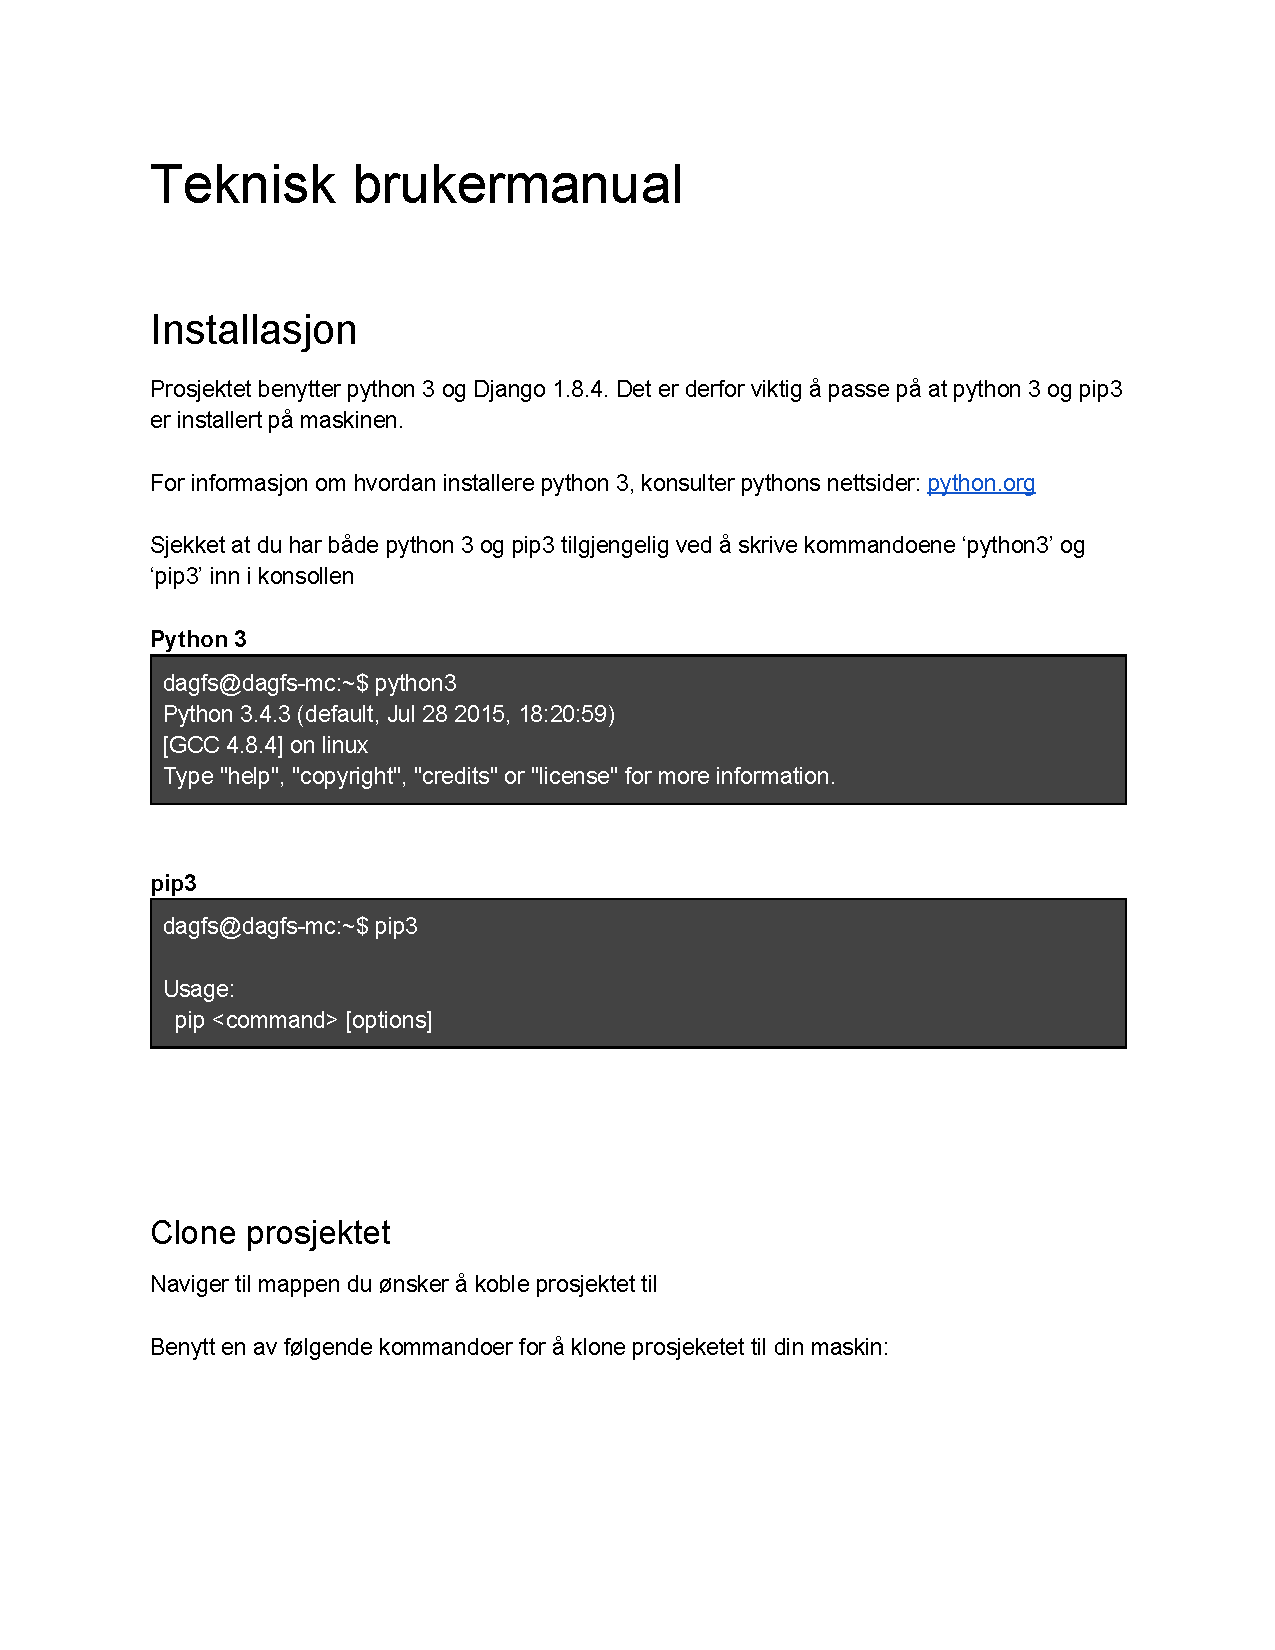
\includepdf[pages={1}, pagecommand={\subsection{Teknisk Brukermanual}}]{vedlegg/tekniskbrukermanual}\label{app:tekniskbrukermanual}
\includepdf[pages={2-}]{vedlegg/tekniskbrukermanual}

%Django
\includepdf[pages={1},pagecommand=\subsection{Django}]{vedlegg/django}\label{app:django}
\includepdf[pages={2-}]{vedlegg/django}

%Task-board
\includepdf[pages={1},pagecommand=\subsection{Taskboard}]{vedlegg/taskboard}\label{app:taskboard}
\includepdf[pages={3-}]{vedlegg/taskboard}

% Risikoanalyse
\includepdf[pages={1},pagecommand=\subsection{Risikoanalyse}]{vedlegg/risikoanal}\label{app:risikoanalyse}
\includepdf[pages={2-}]{vedlegg/risikoanal}

%Motereferanse
\includepdf[pages={1},pagecommand=\subsection{Møtereferat 03.09.2015}]{vedlegg/motereferat0309}\label{app:motereferat0309}
\includepdf[pages={2-}]{vedlegg/motereferat0309}

%Retrospektiv
\subsection{Retrospektiv}\nobreak
    %Todo: Skrive en liten innledning/ forklaring til retrospektiv-sprint...


%Sprint 1
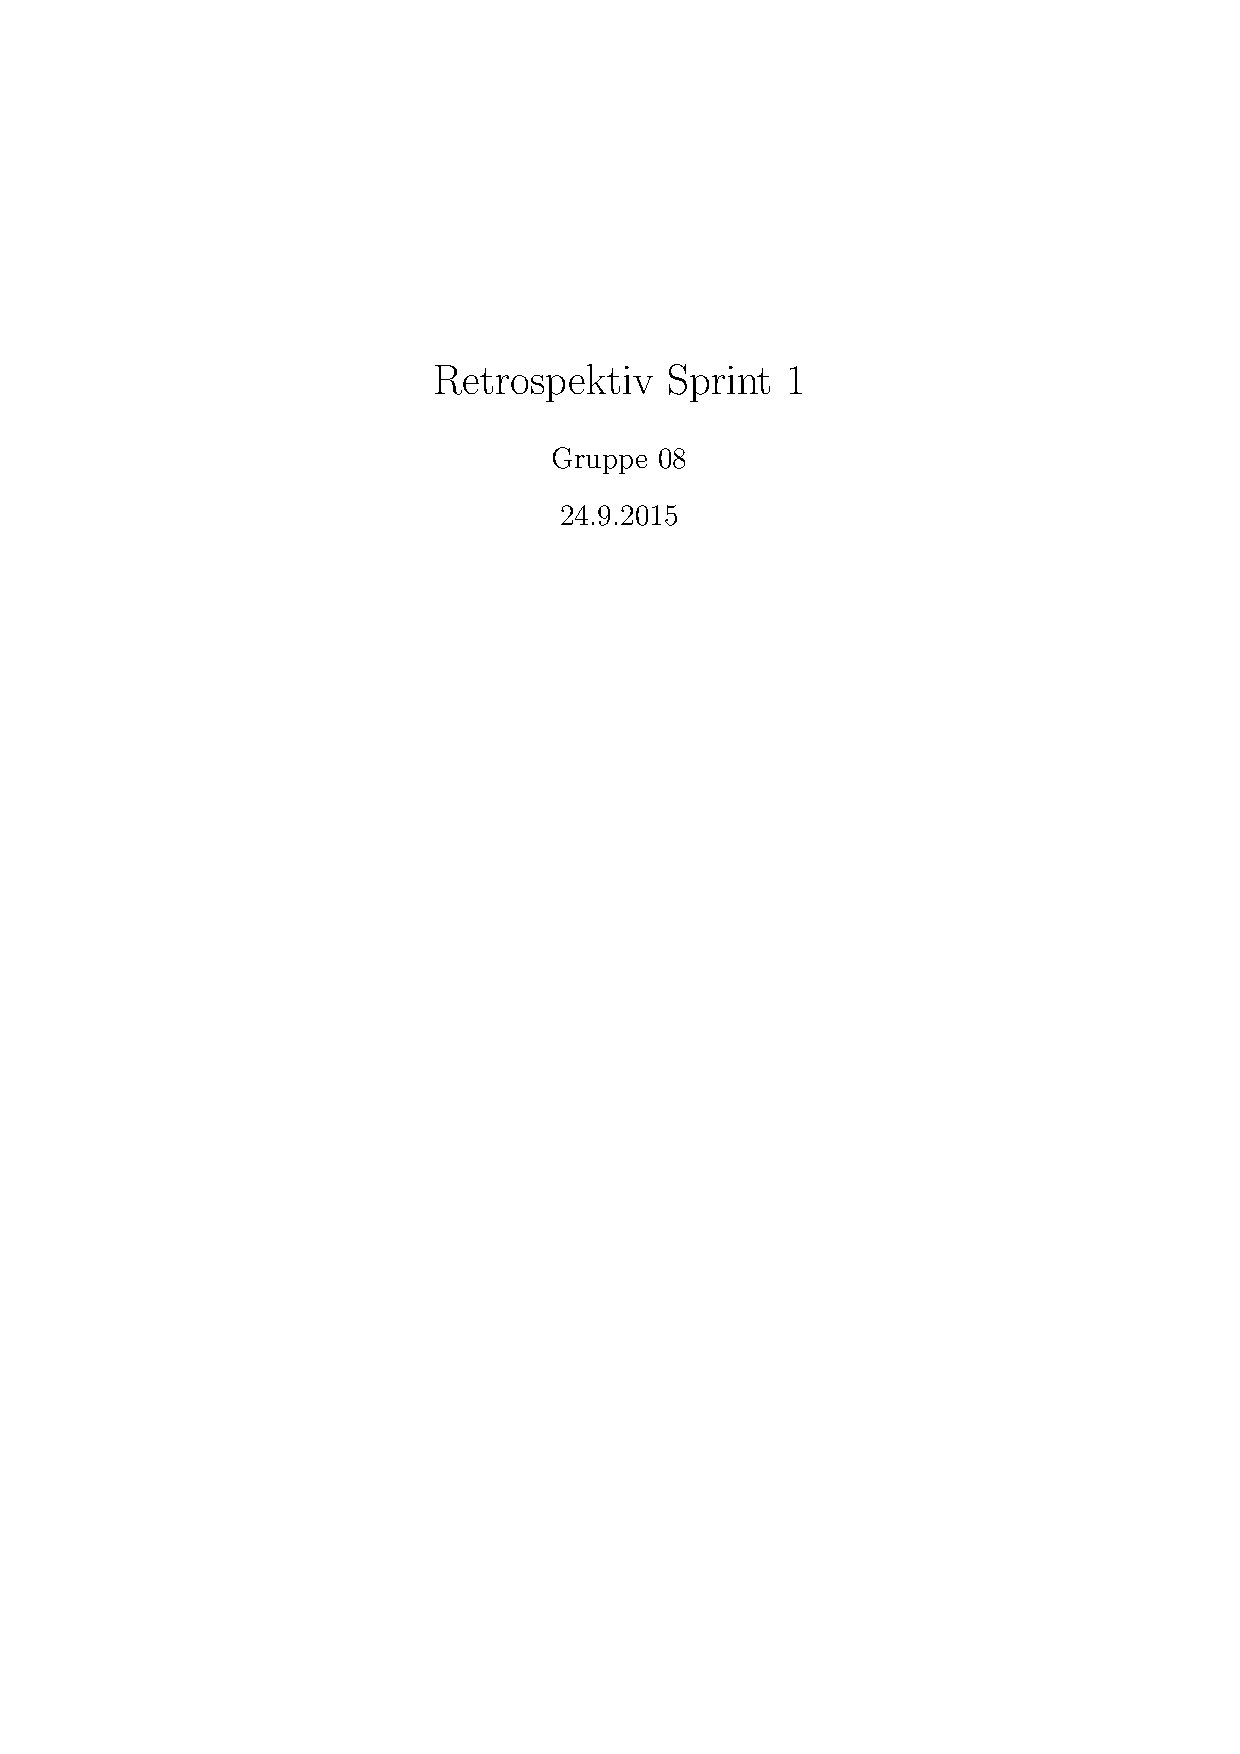
\includepdf[pages={1},pagecommand=\subsubsection{Sprint 1}]{vedlegg/sprint1}\label{app:sprint1}
\includepdf[pages={2-}]{vedlegg/sprint1}

%Sprint 2
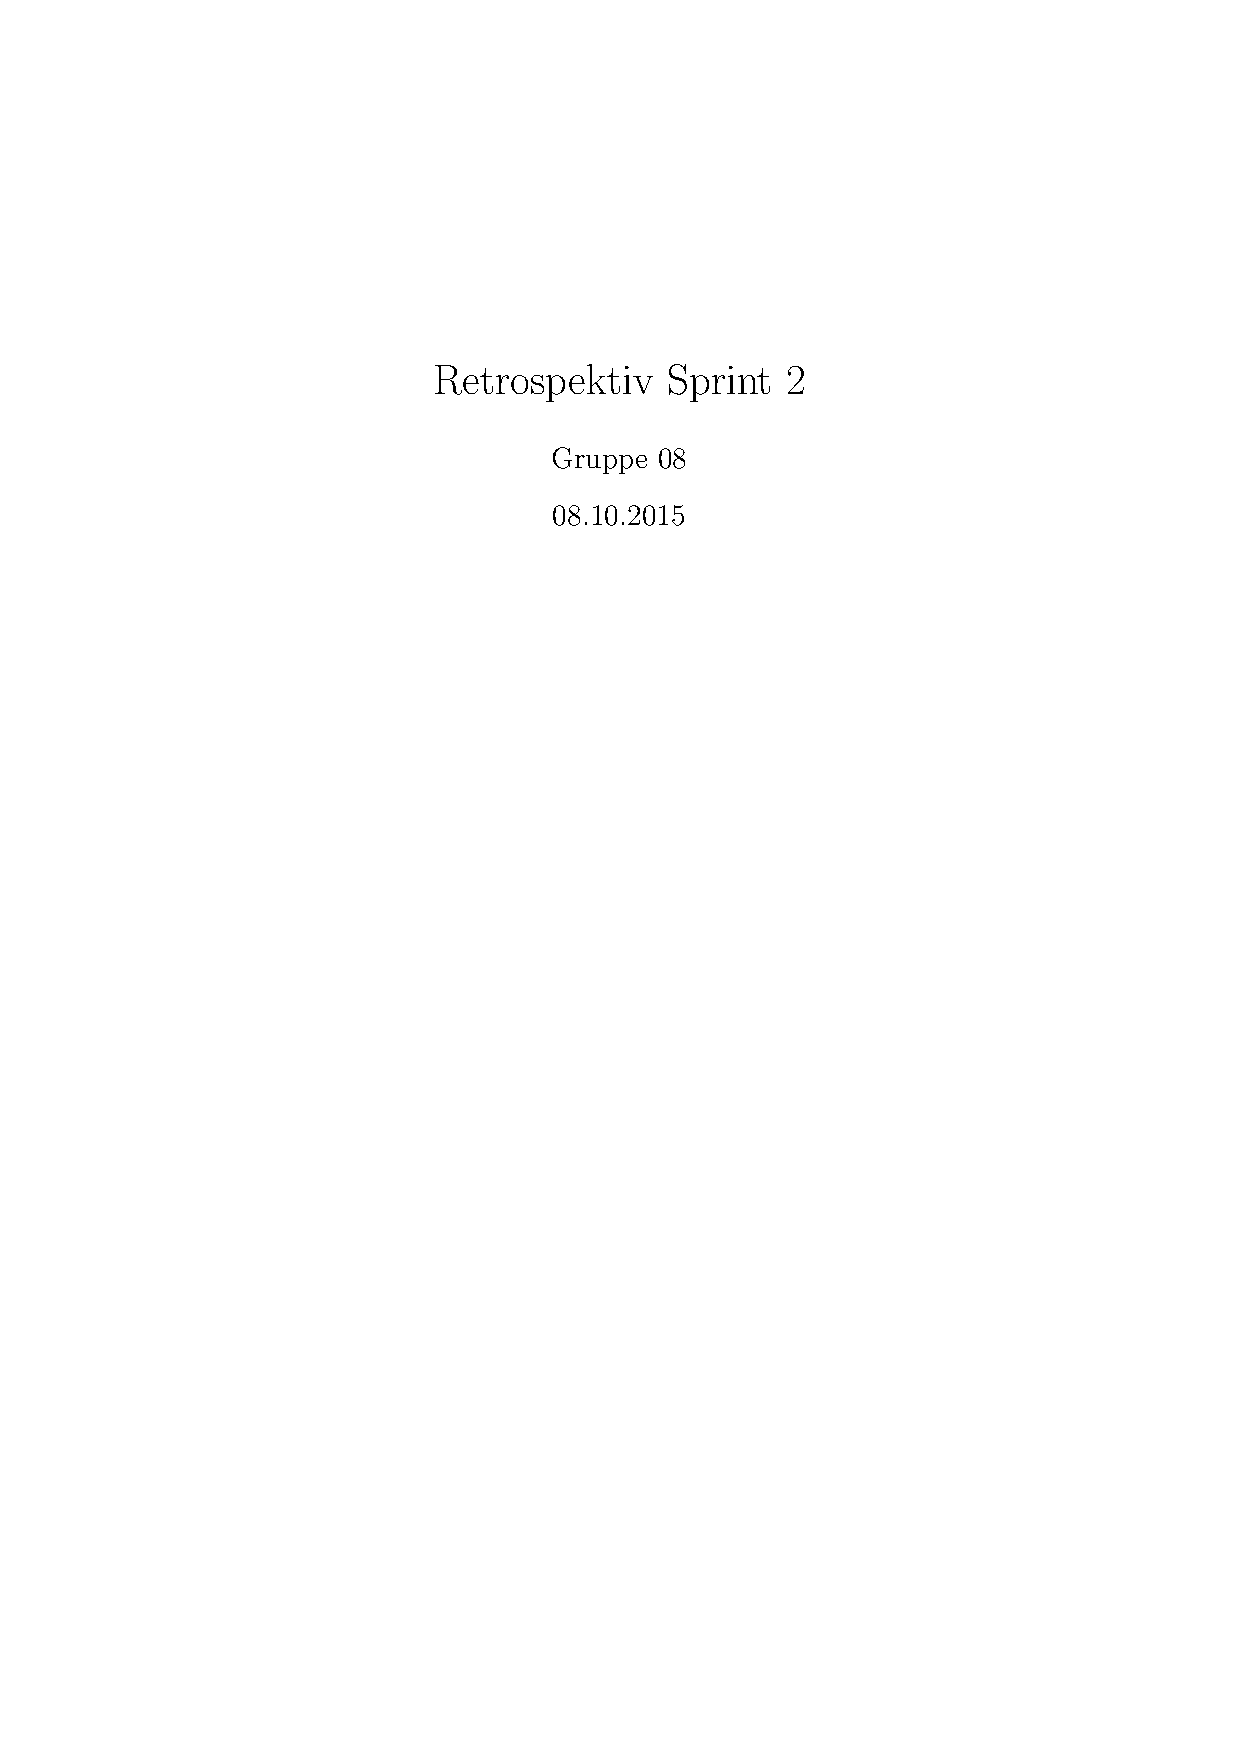
\includepdf[pages={1},pagecommand=\subsubsection{Sprint 2}]{vedlegg/sprint2}\label{app:sprint2}
\includepdf[pages={2-}]{vedlegg/sprint2}

%Sprint 3
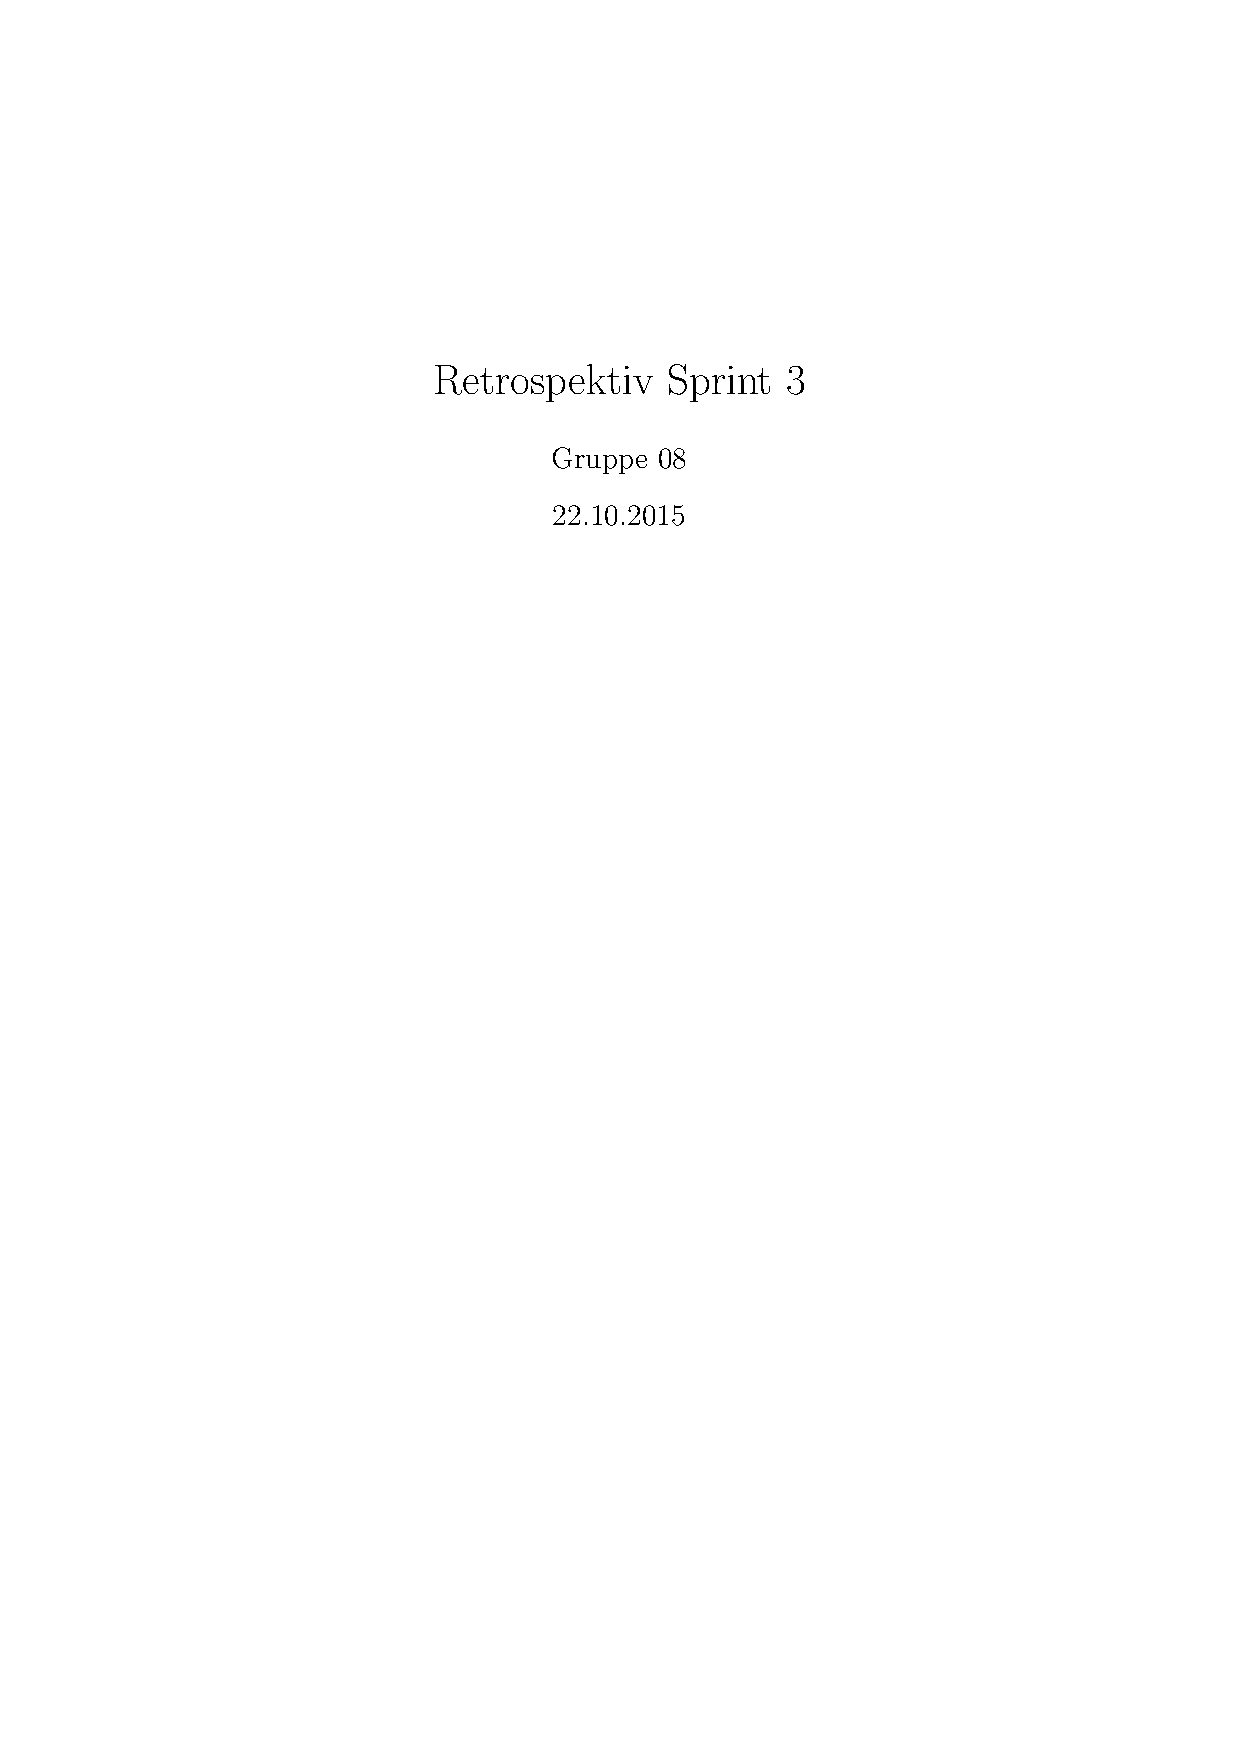
\includepdf[pages={1},pagecommand=\subsubsection{Sprint 3}]{vedlegg/sprint3}\label{app:sprint3}
\includepdf[pages={2-}]{vedlegg/sprint3}

%Sprint 4
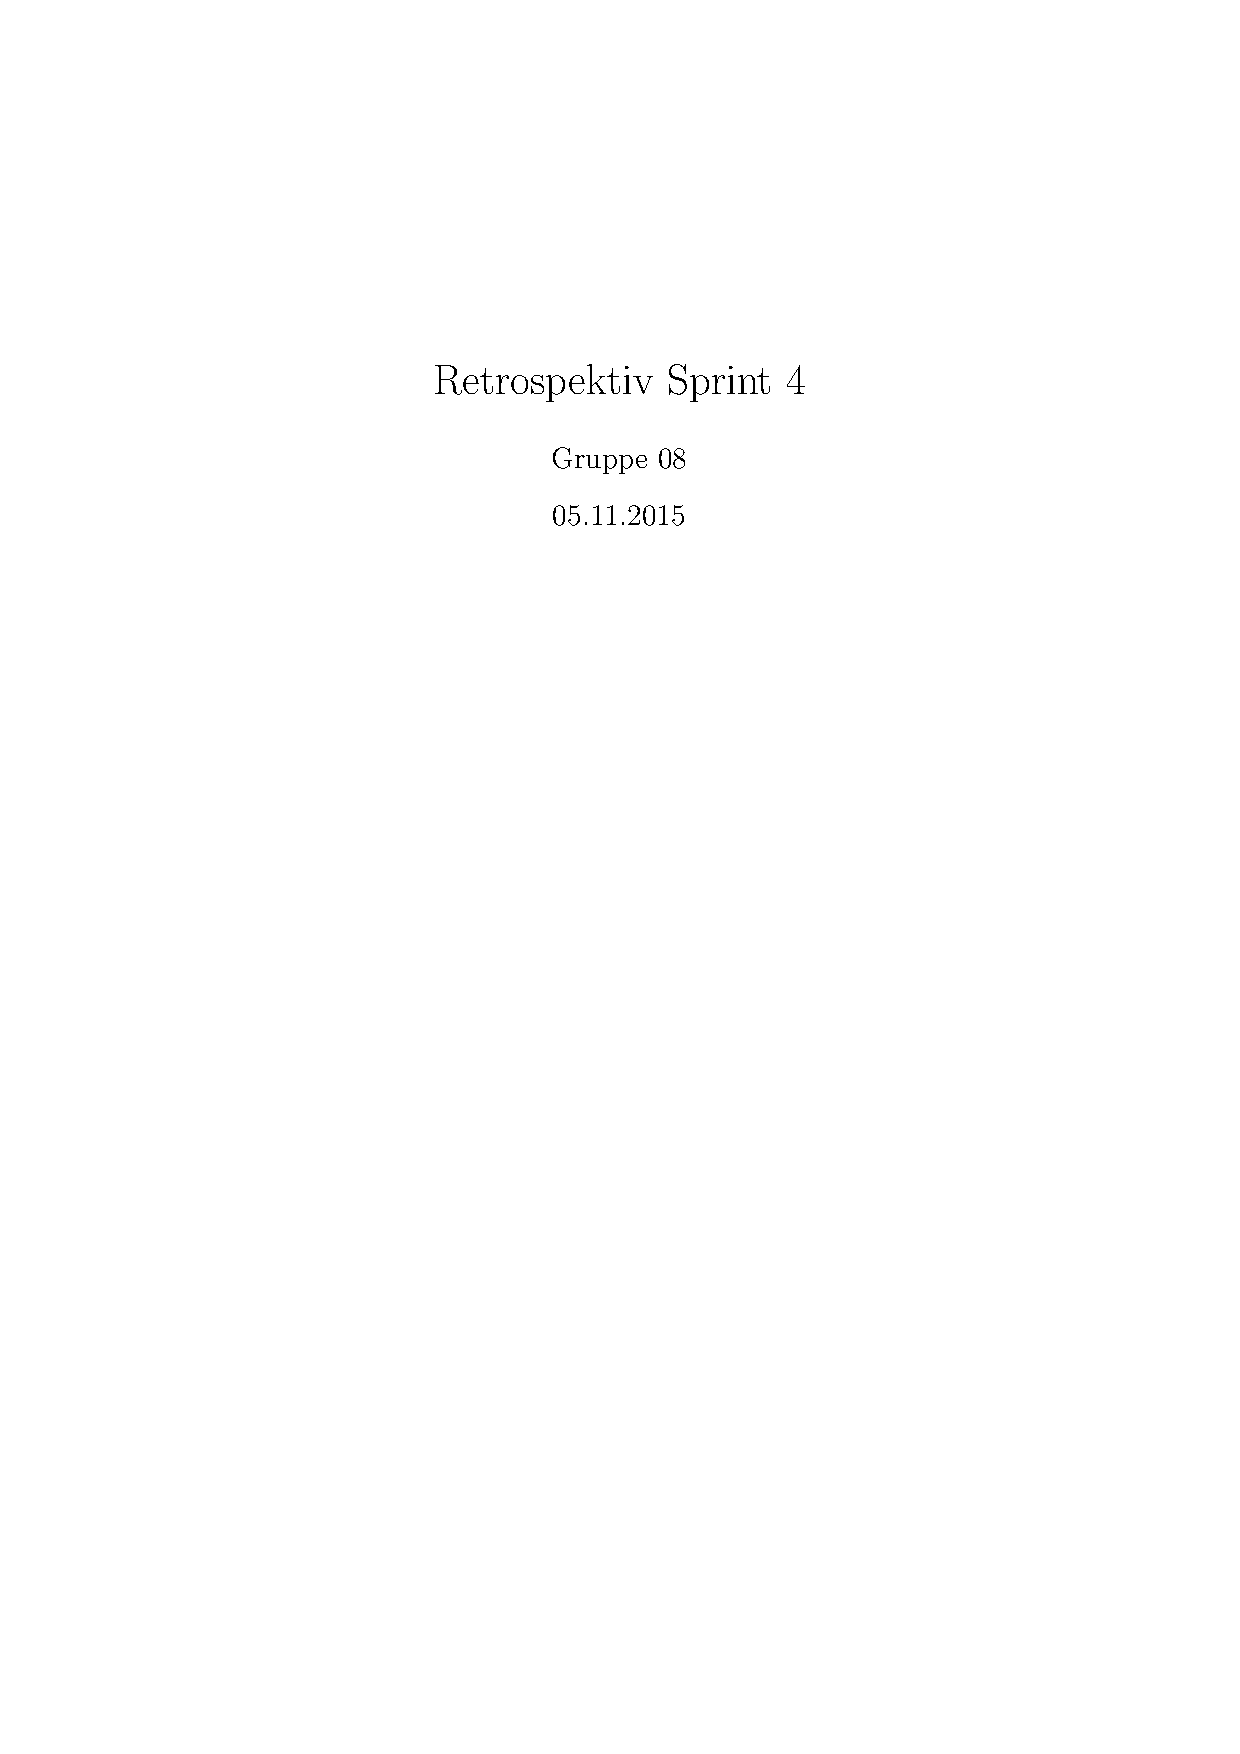
\includepdf[pages={1},pagecommand=\subsubsection{Sprint 4}]{vedlegg/sprint4}\label{app:sprint4}
\includepdf[pages={2-}]{vedlegg/sprint4}

%%RELEASEPLAN
\subsection{Releaseplan}

%¿Hvorfor er disse kommentert ut?
%
\includepdf[pages={1},pagecommand=\subsubsection{Releaseplan-v1}]{vedlegg/releaseP1}\label{app:releaseP1}
%
\includepdf[pages={2-}]{vedlegg/releaseP1}

%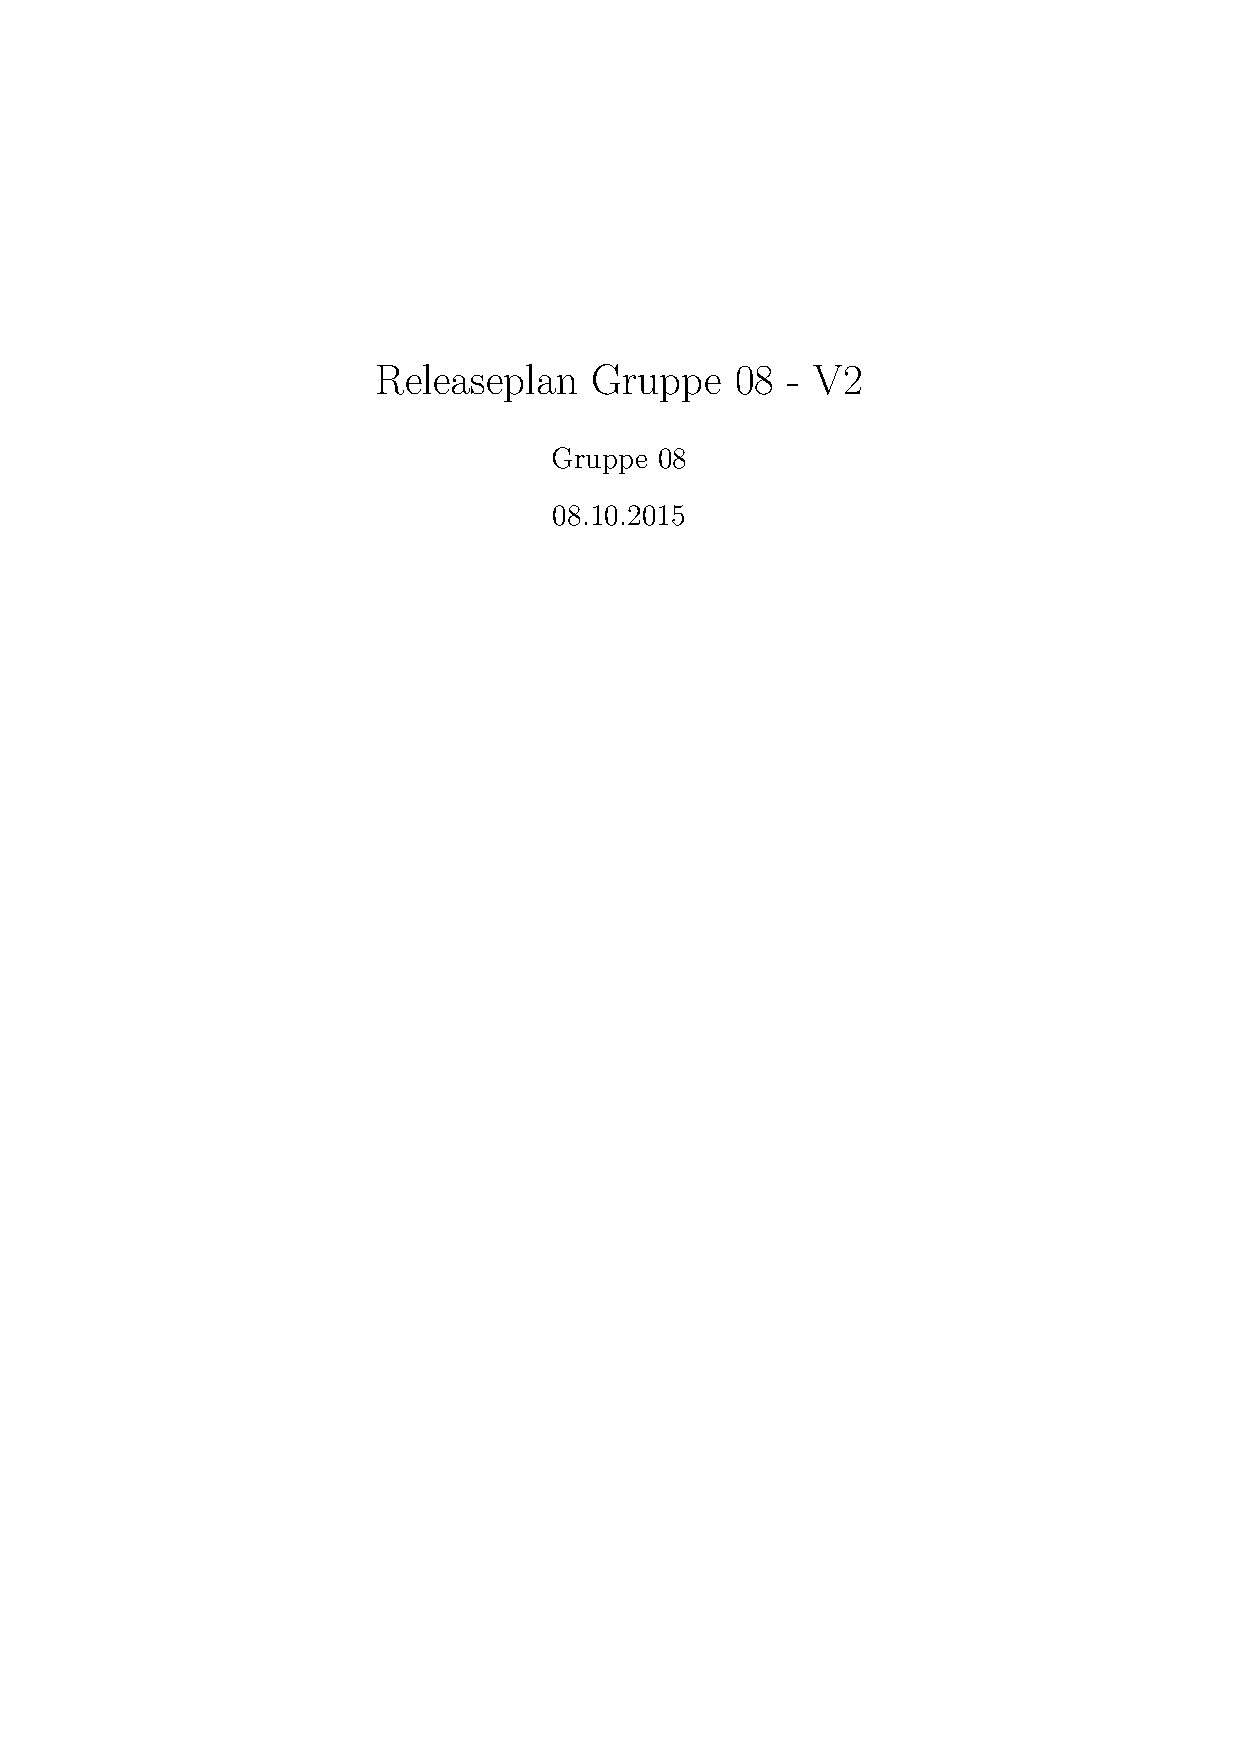
\includepdf[pages={1},pagecommand=\subsubsection{Releaseplan-v2}]{vedlegg/releaseP2}\label{app:releaseP2}
%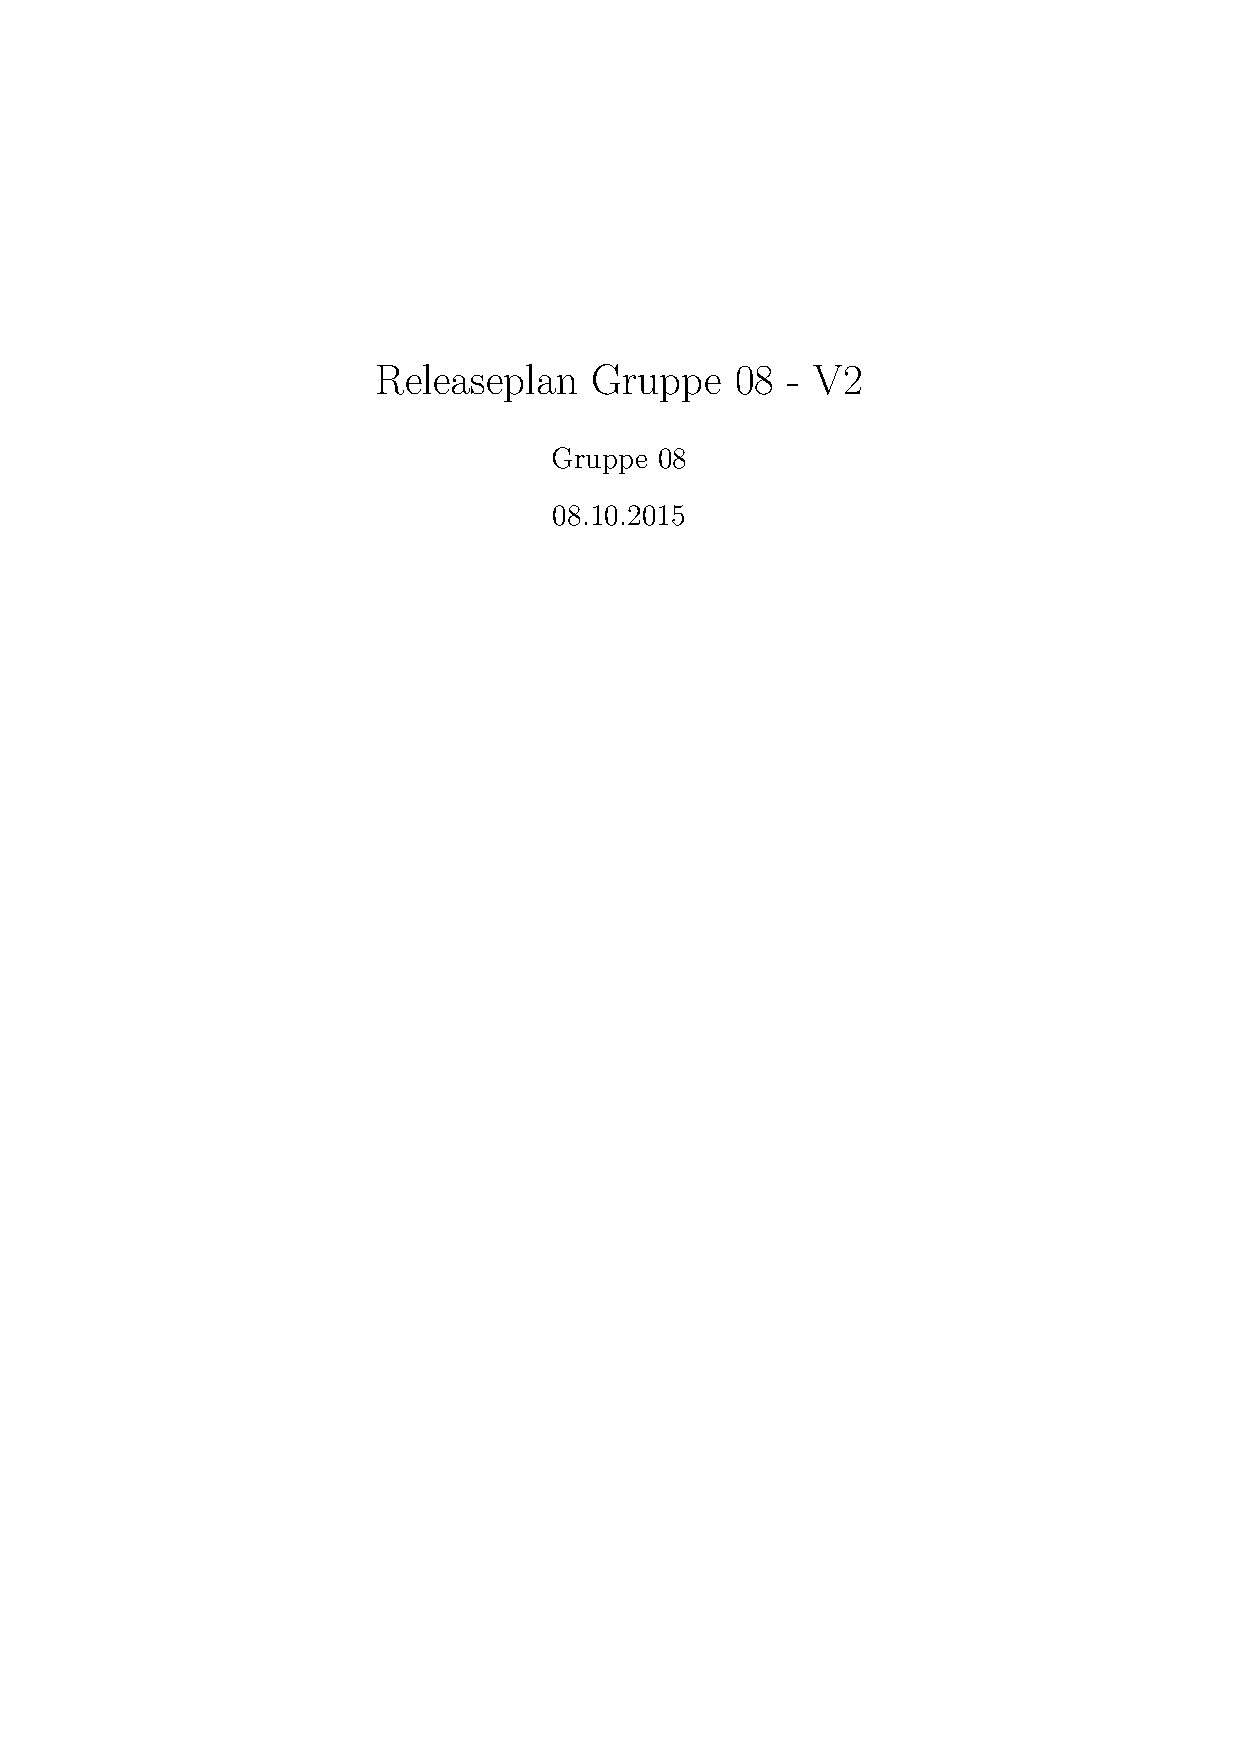
\includepdf[pages={-}]{vedlegg/releaseP2}

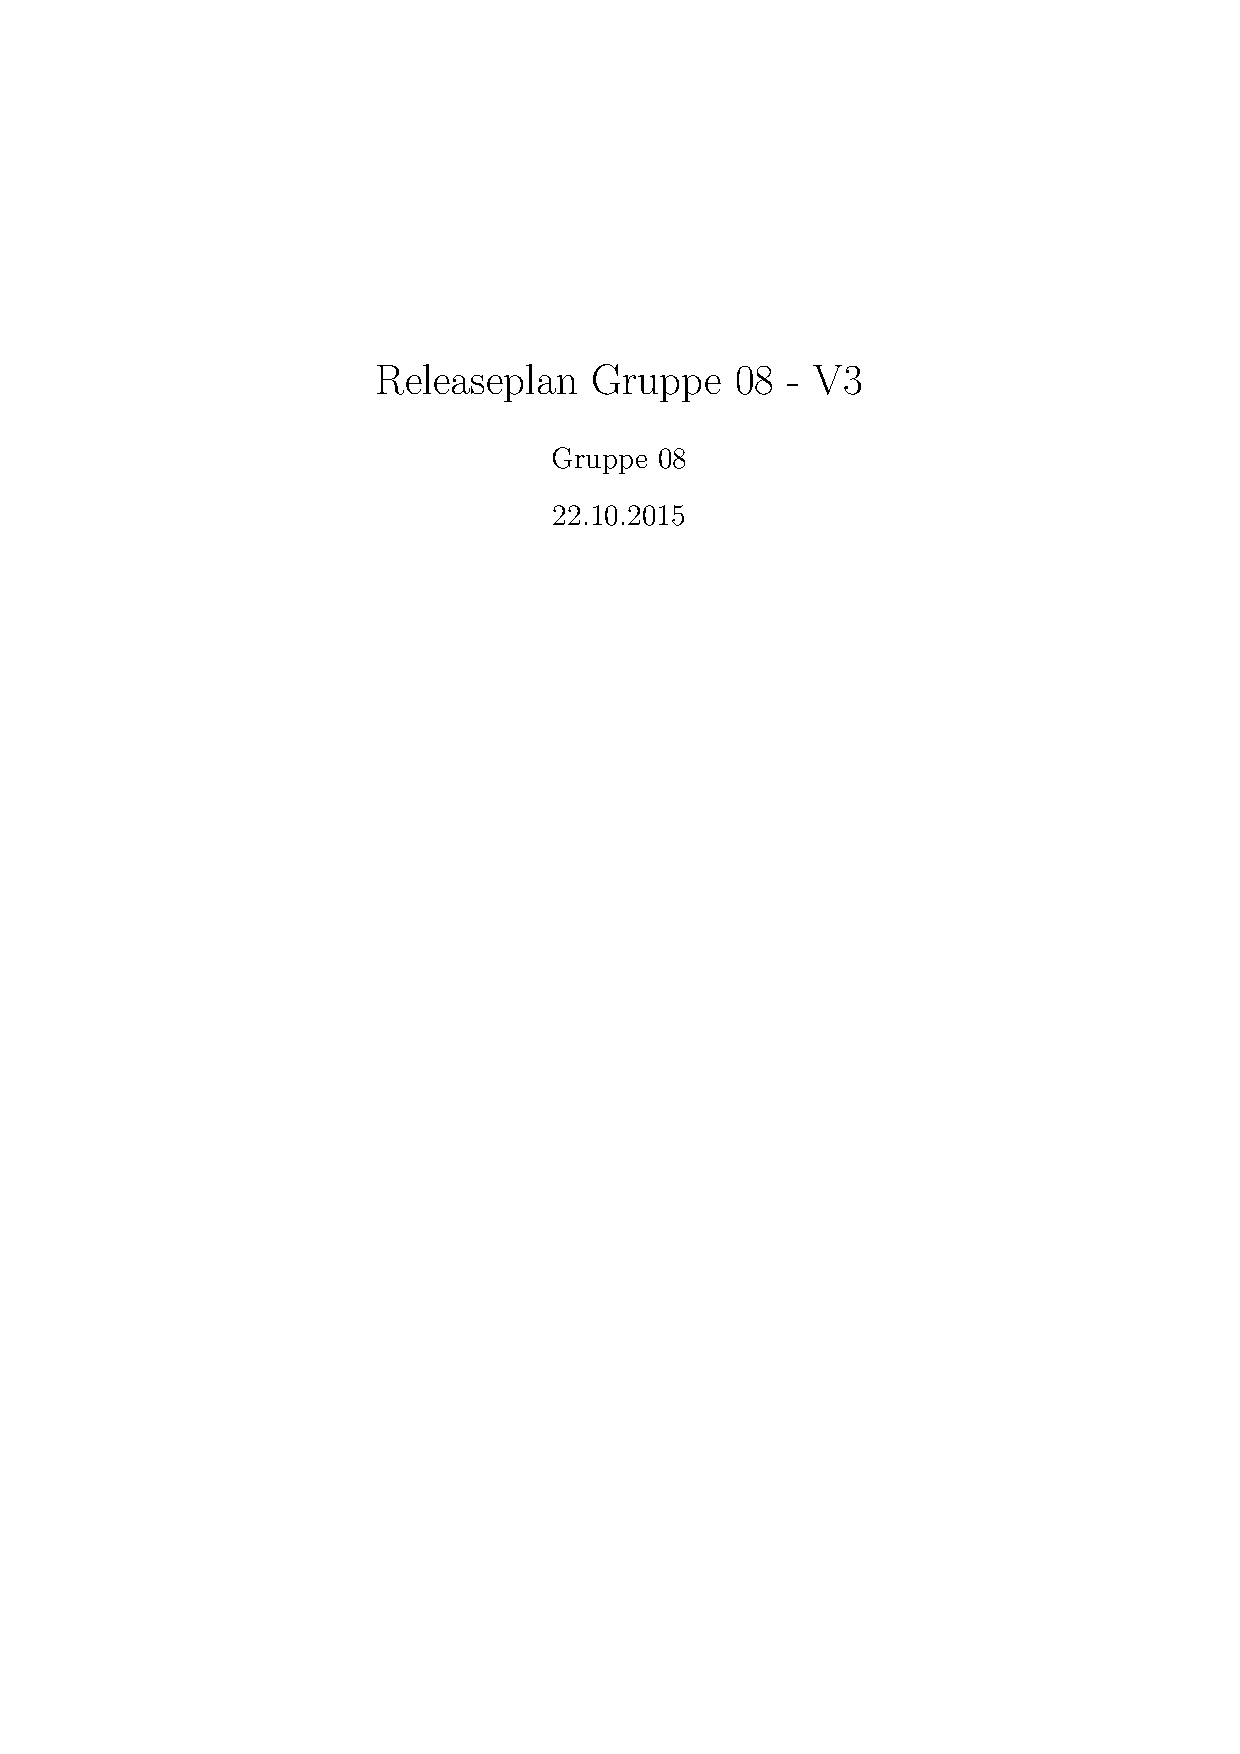
\includepdf[pages={1},pagecommand=\subsubsection{Releaseplan-v3}]{vedlegg/releaseP3}\label{app:releaseP3}
\includepdf[pages={2-}]{vedlegg/releaseP3}

%%Burndown Charts
\subsection{Brenndiagrammer}
\includepdf[pages={1},pagecommand=\subsubsection{Brenndiagram 1}]{vedlegg/burndowncharts}\label{app:brenn}
\includepdf[pages={2-}]{vedlegg/burndowncharts}

\end{appendices}

\end{document}
